\chapter{彭羅斯圖與真實黑洞的形成}

克魯斯卡爾圖景優雅地描述了施瓦西視界附近的區域，但真實黑洞並非永恆存在：它是在物質坍縮時形成的。擴充圖景中有哪些部分能在這段物理歷程中保留下來？要回答這個問題，我們需要一幅足以容納整個時空、又能嚴謹呈現光線運動的圖。我們會先將平直時空緊緻化，再將施瓦西時空緊緻化，最後沿著一層內落的輻射殼層，縫合適當的部分。

\section{視界附近：回顧克魯斯卡爾圖與四個象限}

我們就從上一講結束的地方開始。在施瓦西視界附近，幾何在局部看起來像平直空間。視界本身類似雙曲極座標中的軌跡，就像普通閔可夫斯基時空中的加速座標。在這個局部圖景中，我們從一開始就訂下一條規則，絕不放寬：徑向光線都畫成\(45^\circ\)，而每一條類時世界線都必須比那些類光線更陡。

回顧中的座標，最好理解為內落觀察者所測得的時間與空間。在這組局部慣性座標中，視界附近幾乎是平直的。然而，若觀察者堅持停留在黑洞外的固定半徑處，就不是慣性運動。相對於內落參考系，此人沿著一條加速曲線運動。停留的位置越靠近視界，維持在外所需的加速度就越大。這正是黑板右側那一族外部曲線所呈現的物理意義。

\begin{figure}[htbp]
\centering
\includegraphics[width=0.72\textwidth]{lecture_08_figure_02.png}
\caption{視界附近四區域幾何的黑板草圖。外部的紅色曲線表示一族固定半徑懸停觀察者的世界線。}
\lectureframe{00:02:54}
\end{figure}

\begin{figure}[htbp]
\centering
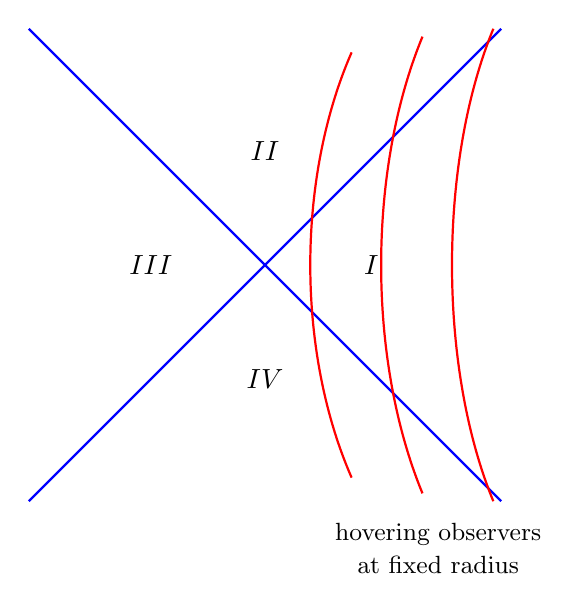
\begin{tikzpicture}[scale=1.0]
\draw[thick,blue] (-3,3) -- (3,-3);
\draw[thick,blue] (-3,-3) -- (3,3);

\draw[red,thick] (1.1,-2.7) .. controls (0.4,-1.1) and (0.4,1.1) .. (1.1,2.7);
\draw[red,thick] (2.0,-2.9) .. controls (1.3,-1.2) and (1.3,1.2) .. (2.0,2.9);
\draw[red,thick] (2.9,-3.0) .. controls (2.2,-1.3) and (2.2,1.3) .. (2.9,3.0);

\node at (1.35,0.0) {$I$};
\node at (0.0,1.45) {$II$};
\node at (-1.45,0.0) {$III$};
\node at (0.0,-1.45) {$IV$};

\node[align=center] at (2.2,-3.6) {\small hovering observers\\\small at fixed radius};
\end{tikzpicture}
\caption{回顧中使用的克魯斯卡爾式因果結構重繪圖。區域\(I\)是外部，區域\(II\)是無法逃離的內部，而區域\(III\)與\(IV\)屬於形式上的延拓；對於真實坍縮形成的黑洞，稍後會捨去這些區域。}
\end{figure}

這已足以說明黑洞如何影響物體與訊號。在外部區域\(I\)，它們可以向內移動，也可以留在外部或折返向外。相較之下，在區域\(II\)，因果結局已經確定：一旦進入內部，就沒有未來指向的因果路徑能返回外部。若要從區域\(II\)逃往任一外部區域，軌跡就必須在某處比\(45^\circ\)更平緩，也就是必須超越光速。所有允許的未來指向類時軌跡，最終都會抵達奇點。

這段開場回顧不只是重複前一講的內容，也為本講的主題作準備。克魯斯卡爾圖景固然有用，但其中並非每一部分都對真實黑洞具有物理意義。

\begin{classroomqa}
\audiencequestion{圖的座標軸代表什麼？紅色曲線是哪種觀察者的固定位置世界線？}
\lecturerresponse{座標軸代表自由落體觀察者所使用的自然座標中的時間與空間。在視界附近，這位觀察者看到的幾乎是普通的平直時空。紅色的定位置曲線則代表被維持在黑洞外、相對靜止的觀察者。這些是加速世界線，而且越靠近視界，所需的加速度越大。
\lecturetimestamp{00:05:58--00:06:47}}
\end{classroomqa}

\section{為何要緊緻化？從無限時空到有限黑板}

接下來要採取的是一種方法上的轉換。這些圖中的類光方向延伸至無窮遠，時間本身也沒有盡頭。因此，若不改變座標，就無法在普通黑板上畫出整個時空。講者的動機很具體：若要一覽全貌並推理全域因果結構，我們就需要一種方法，將無限的時空壓縮至有限區域，同時仍能辨認光線。

因此，他先退回到最簡單的情形，也就是熟悉的平直時空。由於我們關心的問題具有球對稱性，便略去角方向，只保留時間與徑向座標。我們使用座標\(T\)與\(R\)，並令
\[
R\ge 0,
\]
因為在極座標中，負的徑向距離沒有意義。我們也選擇一組單位，使得
\[
c=1.
\]
依照這項約定，徑向類光運動會畫成\(45^\circ\)。

引入緊緻化映射之前，講者先花了一些時間帶我們熟悉\(T\)-\(R\)平面。在圖上畫出時間軸、徑向軸、幾條等時切片\(T=0,\pm1,\pm2\)，以及幾條等半徑線\(R=1,2,3\)。這不是徒具形式的步驟；它提供了參照標記，也讓我們看清楚，稍後將圖壓縮至有限大小時，哪些特徵必須保留。

關於原點，還有一個微妙卻重要的教學要點。在約化的徑向圖中，恰好朝向\(R=0\)的光線看起來像是在原點反彈後折返。但實際上並沒有光線撞上牆壁而反射。在完整的球對稱幾何中，光線只是穿過原點，從另一側出來。這種看似反彈的現象，只是因為我們採用半平面\(R\ge 0\)來描述。

同樣地，沒有正對原點的光線一開始看起來也幾乎相同；它到達最近接近點後，便轉向外側。在這組座標中，甚至可能看起來像是有東西把它從原點推開。但這同樣只是熟悉的角動量障礙在座標中的呈現，並不代表有新的力。講者仔細說明這些例子，是希望聽眾先信任這幅圖，再看他如何變換它。

現在來到關鍵步驟。我們要壓縮並拉伸這幅圖，但有一點必須保持不變：徑向光線仍須是\(45^\circ\)線。這就是緊緻化的核心目的。

\begin{classroomqa}
\audiencequestion{所選的原點在物理上有什麼特殊之處嗎？那些看似彎曲的光線，是原點存在某種力的證據嗎？}
\lecturerresponse{沒有。在這個階段，原點只是球座標選定的中心。看似反彈與彎曲的現象，是把完整的空間運動約化為\(R\geq0\)所造成的。對稱性有時會讓中心成為方便的選擇，例如研究太陽時便是如此；但選擇座標並不會因此在該處放入黑洞或反射牆。
\lecturetimestamp{00:16:27--00:17:08}}
\end{classroomqa}

\section{零座標中的平直時空與彭羅斯形式}

為了精確描述這種變換，我們引入零座標。這是講座中數學處理較為俐落的部分，黑板上的推導清楚呈現了這個步驟。

\begin{figure}[htbp]
\centering
\includegraphics[width=0.82\textwidth]{lecture_08_figure_03.png}
\caption{引入\(T^+=T+R\)與\(T^-=T-R\)時，完整呈現的\(T\)-\(R\)黑板。約化徑向座標的原點就是藍色的垂直線\(R=0\)。}
\lectureframe{00:19:45}
\end{figure}

我們定義
\begin{align}
T^+ &= T+R, \\
T^- &= T-R.
\end{align}
這組座標是為徑向類光運動而設。入射徑向光線滿足\(T^+=\text{const}\)，出射徑向光線則滿足\(T^-=\text{const}\)。

\paragraph{推導。}
在這組座標中，線\(R=0\)的形式特別簡單。事實上，
\begin{align}
R=0
&\iff T+R=T-R \\
&\iff T^+=T^-.
\end{align}
因此，整條類時邊界\(R=0\)都可由單一關係式表示：
\begin{equation}
R=0 \iff T^+=T^-.
\end{equation}

\begin{figure}[htbp]
\centering
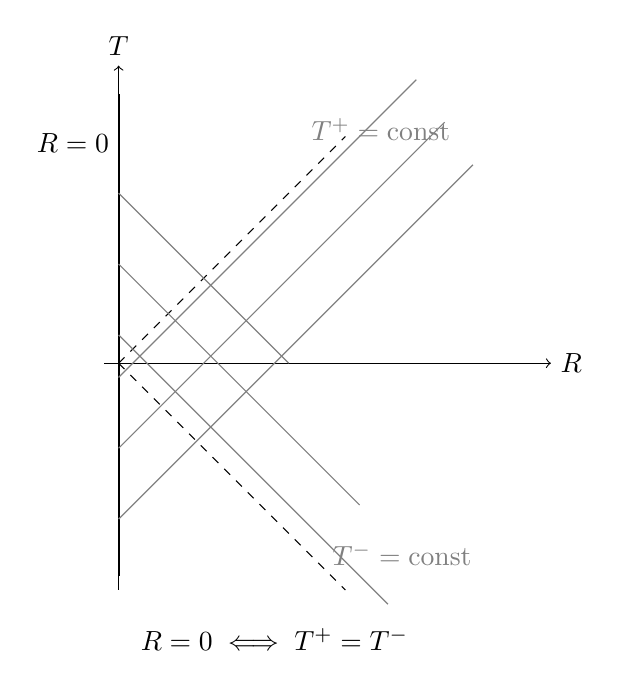
\begin{tikzpicture}[scale=0.9]
\draw[->] (-0.2,0) -- (6.1,0) node[right] {$R$};
\draw[->] (0,-3.2) -- (0,4.2) node[above] {$T$};

\draw[thick] (0,-3.0) -- (0,3.8);
\node[left] at (0,3.1) {$R=0$};

\draw[dashed] (0,0) -- (3.2,3.2);
\draw[dashed] (0,0) -- (3.2,-3.2);

\draw[gray] (0,2.4) -- (2.4,0);
\draw[gray] (0,1.4) -- (3.4,-2.0);
\draw[gray] (0,0.4) -- (3.8,-3.4);

\draw[gray] (0,-2.2) -- (5.0,2.8);
\draw[gray] (0,-1.2) -- (4.6,3.4);
\draw[gray] (0,-0.2) -- (4.2,4.0);

\node[gray] at (3.7,3.3) {$T^+=\mathrm{const}$};
\node[gray] at (4.0,-2.7) {$T^-=\mathrm{const}$};

\node at (2.2,-3.9) {$R=0 \iff T^+=T^-$};
\end{tikzpicture}
\caption{重新繪製的\(T\)-\(R\)平面。兩族類光線分別是\(T^+\)與\(T^-\)的等值線，而線\(R=0\)也可等價地表示為\(T^+=T^-\)。}
\end{figure}

現在進行緊緻化。我們引入兩個新的零座標\(U^\pm\)，各自以同一個有界單調函數\(F\)作用於相應的\(T^\pm\)而得：
\begin{align}
U^+ &= F(T^+), &
U^- &= F(T^-),
\end{align}
其中
\begin{equation}
F(+\infty)=1,
\qquad
F(-\infty)=-1.
\end{equation}
講座中採用的方便選擇是
\begin{equation}
F(x)=\tanh x,
\end{equation}
因此
\begin{equation}
U^+ = \tanh(T^+),
\qquad
U^- = \tanh(T^-).
\end{equation}
雙曲正切並沒有什麼特殊之處；它只是一個極限行為合適的光滑函數，能將無限的座標範圍壓縮至有限範圍。

類光結構之所以得以保留，原因很簡單。若入射徑向光線滿足\(T^+=\text{const}\)，則
\[
U^+=F(T^+)=\text{const},
\]
同樣地，若出射徑向光線滿足\(T^-=\text{const}\)，則
\[
U^-=F(T^-)=\text{const}.
\]
因此，緊緻化分別重新參數化兩個零方向，徑向光線仍然是\(45^\circ\)線。原點線也同樣被清楚地映射過去：
\[
T^+=T^- \Longrightarrow U^+=U^-.
\]

此時，平直時空的無限半平面已被壓縮成有限三角形。接著，講座說明如何判讀三角形的邊界。空間無窮遠收縮為單一點\(i^0\)；未來與過去的類時無窮遠分別是\(i^+\)與\(i^-\)。兩條類光邊界則是\(\mathcal{I}^+\)與\(\mathcal{I}^-\)，通常分別讀作 scri-plus 與 scri-minus，也就是入射與出射光線的起點和終點。

\begin{figure}[htbp]
\centering
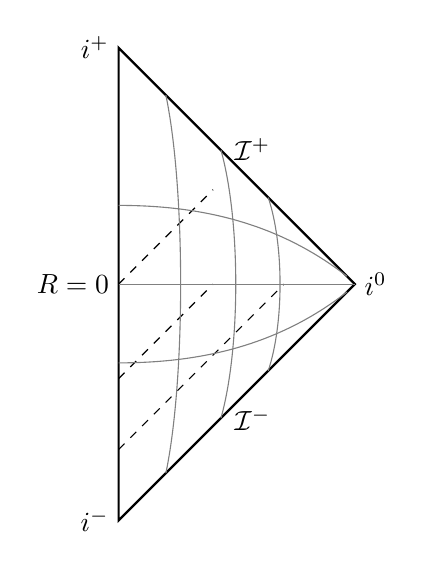
\begin{tikzpicture}[scale=1.0]
\draw[thick] (0,-3) -- (0,3) -- (3,0) -- cycle;

\node[left] at (0,3) {$i^+$};
\node[left] at (0,-3) {$i^-$};
\node[right] at (3,0) {$i^0$};
\node[left] at (0,0) {$R=0$};
\node[above right] at (1.35,1.45) {$\mathcal{I}^+$};
\node[below right] at (1.35,-1.45) {$\mathcal{I}^-$};

\draw[dashed] (0,-2.1) -- (2.1,0.0);
\draw[dashed] (0,-1.2) -- (1.2,0.0);
\draw[dashed] (0,0.0) -- (1.2,1.2);

\draw[gray] (0,0) -- (3,0);
\draw[gray] (0,1.0) .. controls (1.0,1.0) and (2.0,0.8) .. (2.9,0.1);
\draw[gray] (0,-1.0) .. controls (1.0,-1.0) and (2.0,-0.8) .. (2.9,-0.1);

\draw[gray] (0.6,-2.4) .. controls (0.85,-1.2) and (0.85,1.2) .. (0.6,2.4);
\draw[gray] (1.3,-1.7) .. controls (1.55,-0.8) and (1.55,0.8) .. (1.3,1.7);
\draw[gray] (1.9,-1.1) .. controls (2.1,-0.5) and (2.1,0.5) .. (1.9,1.1);
\end{tikzpicture}
\caption{徑向約化平直時空的彭羅斯圖。等時曲線向外延伸至\(i^0\)，等半徑曲線則從\(i^-\)上升至\(i^+\)。}
\end{figure}

講座最後還有一點值得記住：這些圖\emph{並不}保留度規所表示的距離大小，而是保留因果結構。這才是我們要找的不變特徵。

\begin{classroomqa}
\audiencequestion{緊緻化後的等時線應該是直線嗎？}
\lecturerresponse{在所選的映射下，只有對稱切片\(T=0\)是直線。其他等\(T\)曲線都會彎曲，具體形狀則取決於緊緻化函數。即使通常所說的時間仍無界延續，極晚時刻的切片也會愈來愈密集地靠近上方邊界。
\lecturetimestamp{00:29:11--00:30:12}}
\end{classroomqa}

\section{緊緻化的施瓦西幾何}

有了平直時空的構造，我們現在回到黑洞，重做一次同樣的事。我們引入零座標，將無限的座標範圍壓縮至有限圖形，以緊緻化克魯斯卡爾幾何。講者將結果描述為一個斜置的矩形，或近似菱形的因果圖：視界呈現為類光邊界，外部的懸停世界線留在視界之外，而內部區域則終止於一個如今可在圖上看見的奇點。

關鍵的物理要點是：對墜落觀察者而言，奇點\emph{並不}遠在無窮處。一旦越過視界，撞上奇點之前剩餘的固有時是有限的。彭羅斯圖讓這一點一目了然。

視界仍由施瓦西條件判定：
\begin{equation}
1-\frac{2MG}{r}=0
\qquad \Longleftrightarrow \qquad
r=2MG.
\end{equation}
等式\(r=2MG\)標示出施瓦西因子變號的位置。

\begin{figure}[htbp]
\centering
\includegraphics[width=0.72\textwidth]{lecture_08_figure_04.png}
\caption{黑板草圖對照形式延拓圖景與物理上相關的黑洞區域。黑板上清楚標出了紅色的「\emph{奇點}」標示。}
\lectureframe{00:37:59}
\end{figure}

\begin{figure}[htbp]
\centering
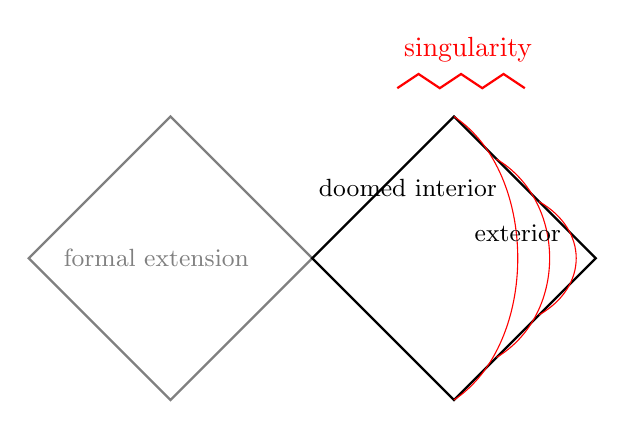
\begin{tikzpicture}[scale=0.9]
\draw[gray,thick] (-4,0) -- (-2,2) -- (0,0) -- (-2,-2) -- cycle;
\draw[thick] (0,0) -- (2,2) -- (4,0) -- (2,-2) -- cycle;

\draw[red,thick] (1.2,2.4) -- (1.5,2.6) -- (1.8,2.4) -- (2.1,2.6) -- (2.4,2.4) -- (2.7,2.6) -- (3.0,2.4);
\node[red] at (2.2,2.95) {singularity};

\draw[red] (2.0,-2.0) .. controls (3.2,-1.2) and (3.2,1.2) .. (2.0,2.0);
\draw[red] (2.6,-1.4) .. controls (3.6,-0.8) and (3.6,0.8) .. (2.6,1.4);
\draw[red] (3.2,-0.8) .. controls (3.9,-0.4) and (3.9,0.4) .. (3.2,0.8);

\node at (2.9,0.35) {\small exterior};
\node at (1.35,1.0) {\small doomed interior};
\node[gray] at (-2.2,0.0) {\small formal extension};
\end{tikzpicture}
\caption{對講座強調的因果圖景所作的審慎重繪：保留下來的外部、無法逃脫的內部、未來奇點，以及它們與形式延拓中額外區域的對照。}
\end{figure}

講者在這裡說得很直接：身處外部，仍有機會逃離，也可能落入黑洞；身處內部，就無法逃脫。這幅圖已經呈現了未來指向因果運動中所有重要的資訊。

象限\(III\)與\(IV\)是最大延拓克魯斯卡爾解中合理的部分。區域\(III\)提供第二個外部，區域\(IV\)則是時間反演後的黑洞區域。然而，這些區域不會出現在一般由坍縮形成的黑洞時空中。延拓解在數學上很有啟發性，因為坍縮構造會顯示哪些部分必須捨去。

\section{空間切片、二維球與愛因斯坦--羅森橋}

現在將緊緻化圖景定格在一個類空切片上，並問：若把它視為\emph{空間}而非時空，它看起來是什麼樣子？這正是蟲洞圖像出現的地方；不過，不能讓空間圖像超越因果論證所能支持的結論。

由於角方向已被省略，徑向圖上的每一點都代表一個二維球。在施瓦西半徑\(r\)處，球面積為
\begin{equation}
A=4\pi r^2.
\end{equation}
因此，類空切片由一族二維球構成，而不只是一條一維曲線。沿著切片移動時，這些球的大小會改變。

遠處的球面很大。向內移動時，球的半徑逐漸縮小，直到在視界處達到最小值：
\begin{equation}
r_{\min}=2MG.
\end{equation}
若繼續穿過形式延拓的部分，球面又會逐漸膨脹，朝向另一側的漸近平坦區域。這就是愛因斯坦--羅森橋的圖像。

\begin{figure}[htbp]
\centering
\includegraphics[width=0.72\textwidth]{lecture_08_figure_05.png}
\caption{延拓克魯斯卡爾圖，以及用來構造橋幾何的綠色類空切片。切片上的每一點都代表一個二維球；其最小半徑標示為\(r=2MG\)。}
\lectureframe{00:41:30}
\end{figure}

黑板只顯示了相關施瓦西因子的一部分：
\begin{equation}
1-\frac{2MG}{r},
\end{equation}
而喉部也出現在同一個特殊半徑\(r=2MG\)處。

\begin{figure}[htbp]
\centering
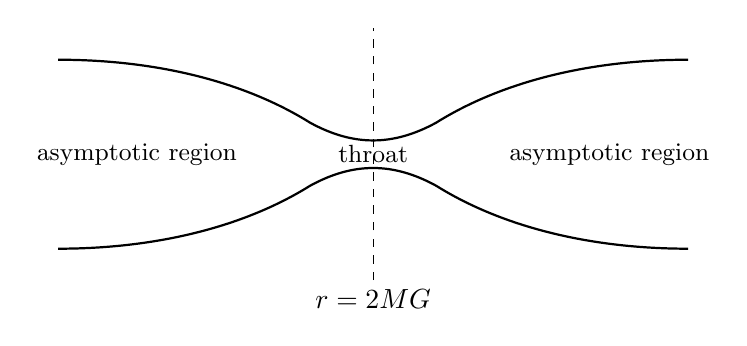
\begin{tikzpicture}[scale=1.0]
\draw[thick] (-4,1.2)
.. controls (-2.7,1.2) and (-1.6,0.9) .. (-0.8,0.4)
.. controls (-0.25,0.1) and (0.25,0.1) .. (0.8,0.4)
.. controls (1.6,0.9) and (2.7,1.2) .. (4,1.2);

\draw[thick] (-4,-1.2)
.. controls (-2.7,-1.2) and (-1.6,-0.9) .. (-0.8,-0.4)
.. controls (-0.25,-0.1) and (0.25,-0.1) .. (0.8,-0.4)
.. controls (1.6,-0.9) and (2.7,-1.2) .. (4,-1.2);

\draw[dashed] (0,-1.6) -- (0,1.6);
\node[below] at (0,-1.6) {$r=2MG$};
\node at (0,0) {\small throat};
\node at (-3.0,0) {\small asymptotic region};
\node at (3.0,0) {\small asymptotic region};
\end{tikzpicture}
\caption{穿過延拓施瓦西幾何的示意性空間切片。這是對講座中橋狀圖像的審慎重建，並非實際的嵌入計算。}
\end{figure}

接著要修正這個圖像帶來的印象。切片看似連接兩個漸近區域，容易讓人以為可以穿過橋頸，從一個宇宙前往另一個宇宙。講座先讓這個想法浮現，接著再用因果結構排除它。若要從一個外部區域到達另一個外部區域，世界線就必須在彭羅斯圖的某處比\(45^\circ\)類光線更平緩。這是不允許的。因此，愛因斯坦--羅森橋無法通行。

講者也強調，空間圖像為何可能造成誤解。它描繪的是\emph{某一時刻的空間}，但可用的因果時間不足以穿越橋體。可以粗略地說，橋在任何東西能通過之前就已開啟又關閉。更直接的做法，是回看彭羅斯圖，從中判讀因果結論。

\section{以內落類光殼層構造真實黑洞}

講座在此完全轉換了問題。我們不再讀取永恆黑洞的性質，而是要構造一個真實的黑洞。

為了簡化問題，我們不考慮內部結構複雜的坍縮恆星，而是假想一層薄的球對稱入射輻射殼層。這是一層光殼，因而以光速向內運動。當半徑小到一定程度，殼層上的能量便會集中到足以形成黑洞。

第二個要素是殼層定理在廣義相對論中的形式。

\paragraph{補充說明。}對於本講所採用的球對稱殼層，內部區域是平直時空，外部區域則是施瓦西幾何。這是講座實際採用的殼層定理，亦即伯克霍夫定理類型的陳述；此處不予證明。

講者先回顧牛頓殼層定理來說明這一點：球殼內部沒有引力場，球殼外部的引力場則與位於中心的點質量所產生的場相同。接著，他以此處所需的形式陳述相應的相對論版本：內部是平直時空，外部是施瓦西幾何。殼層可以運動，這條規則仍然成立。

這些條件已足以構造坍縮時空。殼層本身是類光的，因此必須畫成\(45^\circ\)。這條類光線的一側是平直幾何，另一側是施瓦西幾何。規則可概括為：
\begin{equation}
\begin{aligned}
\text{inside shell} &= \text{flat spacetime},\\
\text{outside shell} &= \text{Schwarzschild geometry}.
\end{aligned}
\end{equation}

接合的步驟因此簡單得幾乎令人意外：

\begin{enumerate}
\item 畫出平直時空的彭羅斯圖，只保留入射殼層內側的區域。
\item 畫出施瓦西時空的彭羅斯圖，只保留同一殼層外側的區域。
\item 捨去不適用的部分。
\item 沿著殼層軌跡，縫合兩個保留下來的部分。
\end{enumerate}

講座在黑板上正是這樣進行：從一幅圖中捨去不適用的一半，再從另一幅圖中捨去不適用的一半，然後沿著殼層將適當的部分接合起來。

\begin{figure}[htbp]
\centering
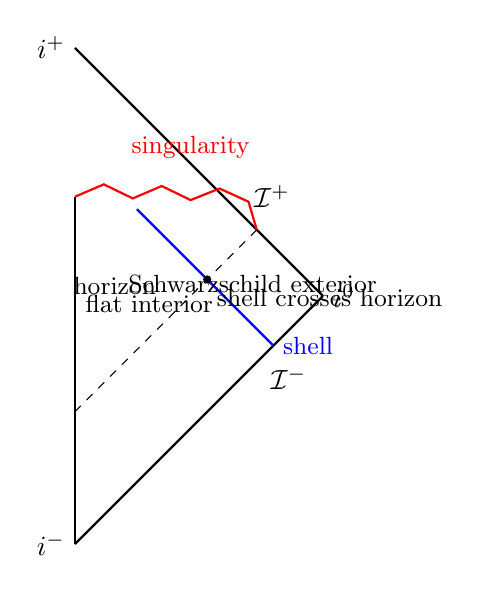
\begin{tikzpicture}[scale=1.05]
\coordinate (im) at (0,-3.0);
\coordinate (ip) at (0,3.0);
\coordinate (i0) at (3.0,0.0);
\coordinate (S)  at (0,1.2);
\coordinate (E)  at (2.2,0.8);
\coordinate (P)  at (2.4,-0.6);
\coordinate (Q)  at (0.75,1.05);
\coordinate (H)  at (0,-1.4);
\coordinate (X)  at (1.6,0.2);

\draw[thick] (im) -- (S);
\draw[thick] (im) -- (i0);
\draw[thick] (ip) -- (i0);

\draw[red,thick] (S) -- (0.35,1.35) -- (0.7,1.18) -- (1.05,1.33) -- (1.4,1.16) -- (1.75,1.30) -- (2.1,1.14) -- (E);
\node[red,above] at (1.4,1.55) {\small singularity};

\draw[thick,blue] (P) -- (Q);
\node[blue,right] at (P) {\small shell};

\draw[dashed] (H) -- (E);
\node[above left] at (1.1,-0.1) {\small horizon};

\filldraw (X) circle (1.2pt);
\node[below right] at (X) {\small shell crosses horizon};

\node at (0.9,-0.1) {\small flat interior};
\node at (2.15,0.15) {\small Schwarzschild exterior};

\node[left] at (im) {$i^-$};
\node[left] at (ip) {$i^+$};
\node[right] at (i0) {$i^0$};
\node[below right] at (2.25,-0.75) {$\mathcal{I}^-$};
\node[above right] at (2.05,0.95) {$\mathcal{I}^+$};
\end{tikzpicture}
\caption{坍縮幾何的因果結構重建。殼層是一條入射類光線；保留其內側的平直時空，以及外側的施瓦西幾何。}
\end{figure}

\begin{figure}[htbp]
\centering
\includegraphics[width=0.76\textwidth]{lecture_08_figure_06.png}
\caption{沿著藍色內落殼層接合平直內部與施瓦西外部後，完成的黑板構造。虛線\(45^\circ\)是從奇點的未來端點向後追蹤，用來找出事件視界。}
\lectureframe{00:57:30}
\end{figure}

殼層從圖中的平直區域進入施瓦西區域時，本身並未經歷任何特殊變化。它是一層類光殼層，會繼續向內，直到抵達奇點。關鍵結構並不在於殼層上發生了什麼局部劇變，而在於接合後時空的因果安排。

\begin{classroomqa}
\audiencequestion{坍縮殼層穿越其施瓦西半徑時，會發生不連續嗎？}
\lecturerresponse{不會。穿越時局部並沒有發生奇異事件。殼層會沿著類光軌跡繼續運動。關鍵在於因果結構：殼層穿過自身的\(2MG\)半徑後，就沒有任何未來指向的路徑能讓它返回無窮遠處。
\lecturetimestamp{00:56:19--00:56:42}}
\end{classroomqa}

\section{視界先於殼層抵達：事件視界之謎}

現在來到講座的概念高潮。坍縮時空構造完成後，自然會問：視界在哪裡？或者如講者所說，不歸點在哪裡？

\paragraph{定義。}事件視界是這樣一道邊界：邊界一側的事件仍能向\(\mathcal{I}^+\)傳送未來指向的因果訊號，另一側的事件則不能。

講座透過圖形找出視界。從奇點與未來類光無窮遠相接的角點出發，沿著\(45^\circ\)類光線向後追蹤。這條向後追蹤的類光線就是事件視界。

接著，講者特別指出第二點，而這正是讓學生感到不安之處：視界並非直到殼層穿過自身的施瓦西半徑時才出現，之後便固定不動。在放大的黑板圖中，視界起初是在中心附近一小片被捕獲區域的邊界，隨後向外延伸，穿過一部分仍然平直的時空，直到較晚才與入射殼層相遇。相遇時，殼層正好穿過自身的施瓦西半徑。從這個事件往上，視界就是已形成黑洞的普通定半徑視界。

\begin{figure}[htbp]
\centering
\resizebox{0.96\linewidth}{!}{%
\begin{tikzpicture}[scale=1.08,>=Latex]
\coordinate (im) at (0,-3.0);
\coordinate (ip) at (0,3.0);
\coordinate (i0) at (3.0,0.0);
\coordinate (S)  at (0,1.2);
\coordinate (E)  at (2.2,0.8);
\coordinate (P)  at (2.4,-0.6);
\coordinate (Q)  at (0.75,1.05);
\coordinate (H)  at (0,-1.4);
\coordinate (X)  at (1.6,0.2);

\draw[thick] (im) -- (S);
\draw[thick] (im) -- (i0);
\draw[thick] (ip) -- (i0);

\draw[red,thick] (S) -- (0.35,1.35) -- (0.7,1.18) -- (1.05,1.33) -- (1.4,1.16) -- (1.75,1.30) -- (2.1,1.14) -- (E);
\node[red,above left] at (S) {\small singularity};

\draw[very thick,red] (H) -- (E);

\draw[thick,blue] (P) -- (Q);

\filldraw (X) circle (1.2pt);

\draw[gray] (0.0,-2.1) .. controls (0.85,-1.95) and (1.9,-1.3) .. (2.8,-0.2);
\draw[gray] (0.0,-1.2) .. controls (0.95,-1.0) and (1.8,-0.45) .. (2.45,0.35);
\draw[gray] (0.0,-0.2) .. controls (0.8,-0.05) and (1.45,0.35) .. (1.95,0.95);

\node[below right] at (2.28,-0.72) {$\mathcal{I}^-$};
\node[above right] at (2.12,0.92) {$\mathcal{I}^+$};

\draw[very thick,red] (3.2,-1.15) -- (3.75,-1.15);
\node[anchor=west] at (3.85,-1.15) {\small event horizon};
\draw[thick,blue] (3.2,-1.55) -- (3.75,-1.55);
\node[anchor=west] at (3.85,-1.55) {\small infalling shell};
\filldraw (3.48,-1.95) circle (1.2pt);
\node[anchor=west] at (3.85,-1.95)
  {\small shell reaches \(r=2MG\)};
\end{tikzpicture}
}
\caption{坍縮圖中以粗線標示向後追蹤的事件視界。視界有一部分位於仍然局部平直、殼層尚未抵達的區域。}
\end{figure}

這個引人注目的效應，是講座接下來著重討論的主題。視界有一部分位於平直時空中。殼層尚未抵達那裡，而且該處甚至不在觀察者的過去光錐上。觀察者感受不到引力場，卻仍然無法逃脫。原因不在於局部的力，而在於該事件的全域因果未來。

\begin{classroomqa}
\audiencequestion{這個構造表示人不能穿越殼層，還是不能穿越視界？當視界仍在殼層內側時，殼層位於哪裡？}
\lecturerresponse{人可以穿越殼層。視界是另一個類光曲面，界定了哪些事件能與\(\mathcal I^+\)通訊、哪些不能。入射殼層正是在穿越與其總能量相對應的施瓦西半徑時，遇上這道邊界。在兩者相遇之前，事件視界有一部分穿過平直的內部；相遇之後，殼層便位於已形成的黑洞內部。
\lecturetimestamp{00:58:42--01:01:06}}
\end{classroomqa}

\begin{classroomqa}
\audiencequestion{如果內部是平直的，而且殼層還在遠處，為什麼剛好位於視界內的人不能在殼層抵達前穿越視界？}
\lecturerresponse{畫出最快可能向外運動的世界線，也就是一條\(45^\circ\)光線。從向後追蹤所得的視界內側某個事件出發，即使這條光線也會太晚才遇上入射殼層，最後仍會抵達奇點。步行只會更慢。「\emph{殼層還沒穿過}」這種說法若沒有先選定時間座標，就不完整；因果圖提供了不依賴座標的答案。入射的宇宙微波背景輻射不是同一個例子，因為它並非造成這種幾何的坍縮球殼。
\lecturetimestamp{01:01:07--01:04:03}}
\end{classroomqa}

\section{鏡子與改變未來的嘗試}

接下來的問題把這幅圖變成了思想實驗室。假設入射光殼能在受困之前被反射，那麼原先假設的坍縮歷程就會改變，事件視界也會隨之改變。這並不矛盾：只有在完整的時空歷程確定後，事件視界才有定義。

\begin{classroomqa}
\audiencequestion{如果在預期的施瓦西半徑外側放置一面完美反射鏡，讓殼層反彈並向外離開，會怎麼樣？}
\lecturerresponse{在這個理想化的歷程中，入射類光線會在鏡面處轉向外側，並抵達未來邊界；原圖中的黑洞便不會形成。真正無重量的鏡子並不存在，而且實際的鏡子本身也會貢獻應力能量；不過，這個思想實驗點出了關鍵：只有在殼層穿過實際的事件視界之後，逃離才不再可能。
\lecturetimestamp{01:04:33--01:05:54}}
\end{classroomqa}

\begin{classroomqa}
\audiencequestion{如果觀察者知道殼層即將到來，能否及時送出鏡子或訊號，讓殼層折返？}
\lecturerresponse{只有在必要的裝置能及早送到視界外側時才行。Alice 可以事先安排 Bob 發送殼層，因此在親眼看見它之前，就知道它即將到來。然而，一旦她所在的事件位於視界內，鏡子或指令都無法及時抵達所需的外部位置。知道未來將進行什麼實驗，並不會打開因果圖所禁止的路徑。
\lecturetimestamp{01:05:55--01:08:18}}
\end{classroomqa}

\begin{classroomqa}
\audiencequestion{已經位於視界內的鏡子會怎麼樣？奇點是否在它未來的無窮遠處？}
\lecturerresponse{鏡子只是另一個注定無法逃脫的物體。它或許能在局部反射光，但反射光、鏡子和 Alice 最終都會抵達奇點。一般的內落世界線會在有限固有時內抵達奇點；只有緊緻化圖中理想化的上方角點才位於無窮遠處。若要試圖留在該角點附近，就需要無界增大的加速度與能量；此外，對於一對固定事件，加速時鐘累積的固有時比慣性時鐘少，而非更多。
\lecturetimestamp{01:08:19--01:10:19}}
\end{classroomqa}

\begin{classroomqa}
\audiencequestion{如果坍縮殼層非常巨大，位於殼層內側、但遠離它最終中心的人，能否在殼層經過時留在原地？}
\lecturerresponse{可以，只要此人所在的事件仍在事件視界之外。位於物質殼層內側，不等於位於黑洞內部。輻射可能撞擊並傷害觀察者，但那是與殼層的局部交互作用，和能否逃脫的因果問題是兩回事。
\lecturetimestamp{01:10:21--01:11:24}}
\end{classroomqa}

\section{時間切片與逐漸擴大的視界}

彎曲時空中的\emph{某一時刻}，指的是選定的一個類空超曲面。這樣一族曲面稱為葉狀分層；為每個曲面指定一個數值，就定義了時間座標。不同的葉狀分層會以不同方式切割同一幅坍縮圖。它們對哪些遙遠事件彼此同時的判定不同，但不會改變哪些零射線能到達無窮遠。

\begin{figure}[htbp]
\centering
\includegraphics[width=0.77\textwidth]{lecture_08_figure_07.png}
\caption{黑板後期的圖，畫有數個綠色類空切片。這些切片提供時間座標；黑色零邊界及其因果關係則不受這項選擇影響。}
\lectureframe{01:17:30}
\end{figure}

\begin{classroomqa}
\audiencequestion{能否把這個謎題重新表述為：在同一時刻，比較觀察者到視界的距離，以及視界到殼層的距離？}
\lecturerresponse{選定葉狀分層後，這種說法有助於建立直覺，但\emph{同一時刻}這個說法取決於座標。更清楚的做法是畫出一族類空切片。早期切片與一個大殼層相交，中央尚無受困區域；較晚的切片則與仍在內落的殼層內部、正在增長的視界相交；其中有一個特定切片通過殼層越過自身施瓦西半徑的事件。
\lecturetimestamp{01:11:26--01:14:21}}
\end{classroomqa}

\begin{classroomqa}
\audiencequestion{視界向外擴展時，施瓦西半徑會隨之增大嗎？殼層越過視界後，視界為什麼還會繼續增長？}
\lecturerresponse{最終的施瓦西半徑\(2MG\)是固定的，因為總質量\(M\)固定不變。早期類空切片上增長的是視界截面的面積半徑。它從中心開始增大，直到在\(r=2MG\)處與殼層相交，隨後便停止增長。在相交事件之上，視界沿著\(r\)保持為\(r=2MG\)的線延伸，儘管共形緊緻化並未使這條線看起來垂直，或在度規上均勻。
\lecturetimestamp{01:14:22--01:16:15}}
\end{classroomqa}

\begin{classroomqa}
\audiencequestion{一位起初位於最終施瓦西半徑一半處的觀察者會遭遇什麼？該觀察者不是應該等到殼層到達時才感受到引力嗎？}
\lecturerresponse{正是如此。觀察者首先在仍處於平坦時空時越過正在增長的事件視界，不會感受到任何突如其來的力。內落的輻射殼層是實在的物質，之後可能會被感受到；事件視界則不是。越過事件視界只表示，從此以後，所有未來指向的因果路徑都無法抵達無窮遠。就這個精確的意義而言，視界有如幽靈。
\lecturetimestamp{01:16:17--01:17:45}}
\end{classroomqa}

\begin{classroomqa}
\audiencequestion{如果觀察者夠早出發，能否向外移動得比正在增長的視界更快，從而逃脫？}
\lecturerresponse{視界之外的事件有通往\(\mathcal I^+\)的向外因果路徑；視界之內的事件則沒有。在選定的切片上，可以比較可用的徑向距離，以及入射殼層封閉逃逸路徑前所剩的時間；但精確的判準是零線。沒有觀察者會看見一個實體視界向外急速擴展，因為當地並不存在可供觀察的表面。
\lecturetimestamp{01:17:46--01:18:54}}
\end{classroomqa}

\section{圖所保留的內容}

不能把圖上的形狀看成按比例繪製的圖。一個小角落可能代表時空中的無限區域，而一大片區域可能只代表有限的物理間隔。共形緊緻化刻意犧牲度規尺度，以保留零方向。保留下來的是因果關係：誰能向誰傳送訊號，哪些事件能影響其他哪些事件，以及哪些世界線受困於光速限制之下。

\begin{classroomqa}
\audiencequestion{如果這幅圖把長度和時間扭曲得如此嚴重，它究竟忠實呈現了什麼？}
\lecturerresponse{它呈現光線，因此也呈現因果結構。要找出事件視界的位置，就從未來無窮遠反向追蹤最後一條向外傳播的零射線。試圖根據圖上看似的距離推斷答案並不可靠。因果圖一旦畫出，關於訊號、逃脫和無法返回的問題就有了幾何上的答案，即使度規尺度已被壓縮也是如此。
\lecturetimestamp{01:18:56--01:21:45}}
\end{classroomqa}

\begin{classroomqa}
\audiencequestion{要花多久才能熟悉彭羅斯圖，進而憑直覺運用它們？}
\lecturerresponse{不需要很久。實際做法是畫圖、追蹤零線，並檢驗可能的世界線，直到熟悉其中的因果限制。這裡的直覺是透過實際運用圖形培養出來的，而不是不看圖就憑空猜測。
\lecturetimestamp{01:21:49--01:22:05}}
\end{classroomqa}

\begin{classroomqa}
\audiencequestion{這種視覺化方法是否與量子力學相反？在量子力學中，數學往往比圖像更可靠。}
\lecturerresponse{在很大程度上，是的。廣義相對論是經典物理學。四維彎曲時空很難直接想像，彭羅斯圖本身也仍然抽象；然而，因果幾何可以透過圖形描繪並加以探索，其程度遠勝於量子力學底層實在所能達到的程度。這種差異正是彭羅斯圖如此有力的原因之一。
\lecturetimestamp{01:22:05--01:22:58}}
\end{classroomqa}